\chapter{Supplementary material on timeseries data}

\section{Further examples of trajectory data}

Find below the trajectory timeseries visualisation plots - as figure 4.2 - for the locations in figure 4.1. Each figure contains plots (a-d) of TX1day T’ decompositions for years 1980 to 2020. The x-axis is logarithmic to better represent the recent
 history. The trajectory yielding the largest final T’ among all years is colored red, the
 time-mean of all trajectories in black and the inter-quantile range is highlighted in light
 blue. It also contains the average auto-correlation (e) and cross-correlation with T’ (f) over all events
 for each contributor. The auto- and cross-correlation are computed for timeseries starting
 at genesis (ignoring padding) and timeseries that are smaller than 32 timesteps are not
 included in the averages for lags larger than their length.

\begin{figure}[h]
\caption{Location 28.5N 77E, in the vicinity of New Delhi, India.}
\centering
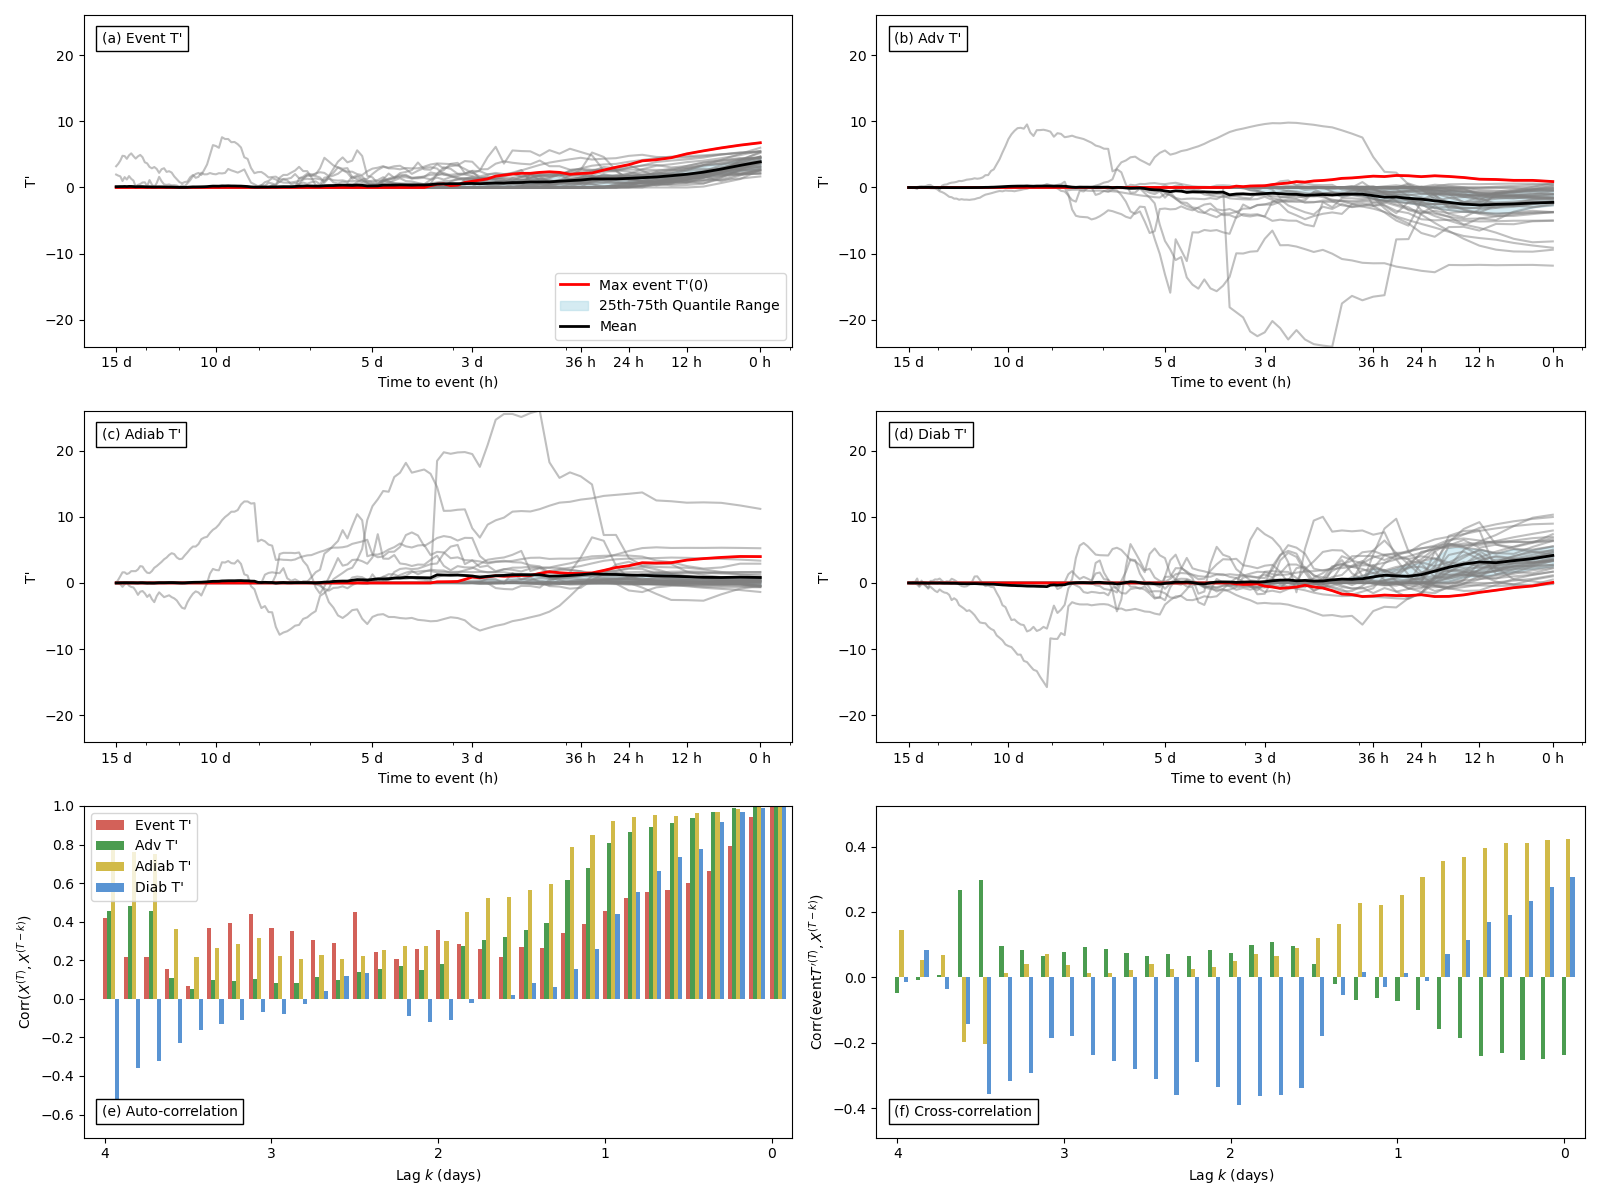
\includegraphics[width=0.9\textwidth]{images/sup1.png}
\end{figure}

\begin{figure}[h]
\caption{Location 45N 30W, in the middle of the Atlantic ocean.}
\centering
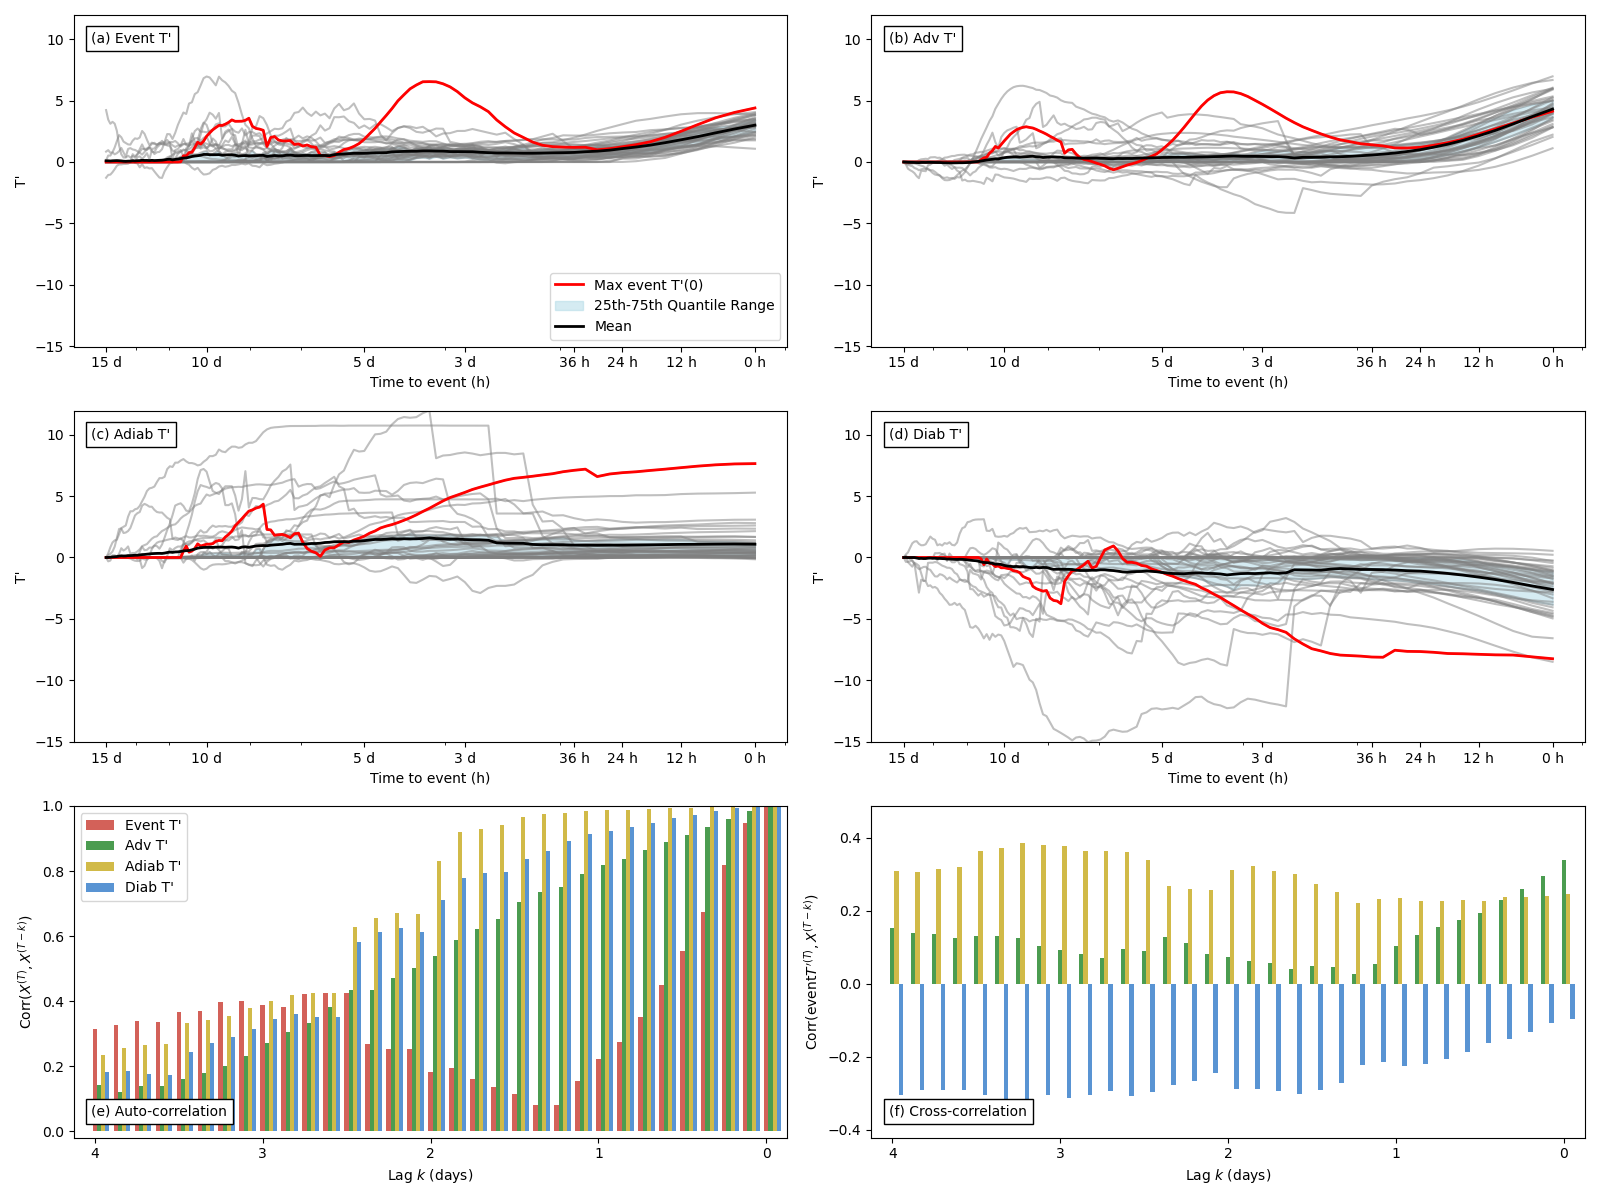
\includegraphics[width=0.9\textwidth]{images/sup2.png}
\end{figure}

\begin{figure}[h]
\caption{Location 32S 116E, in the vicinity of Perth, Australia.}
\centering
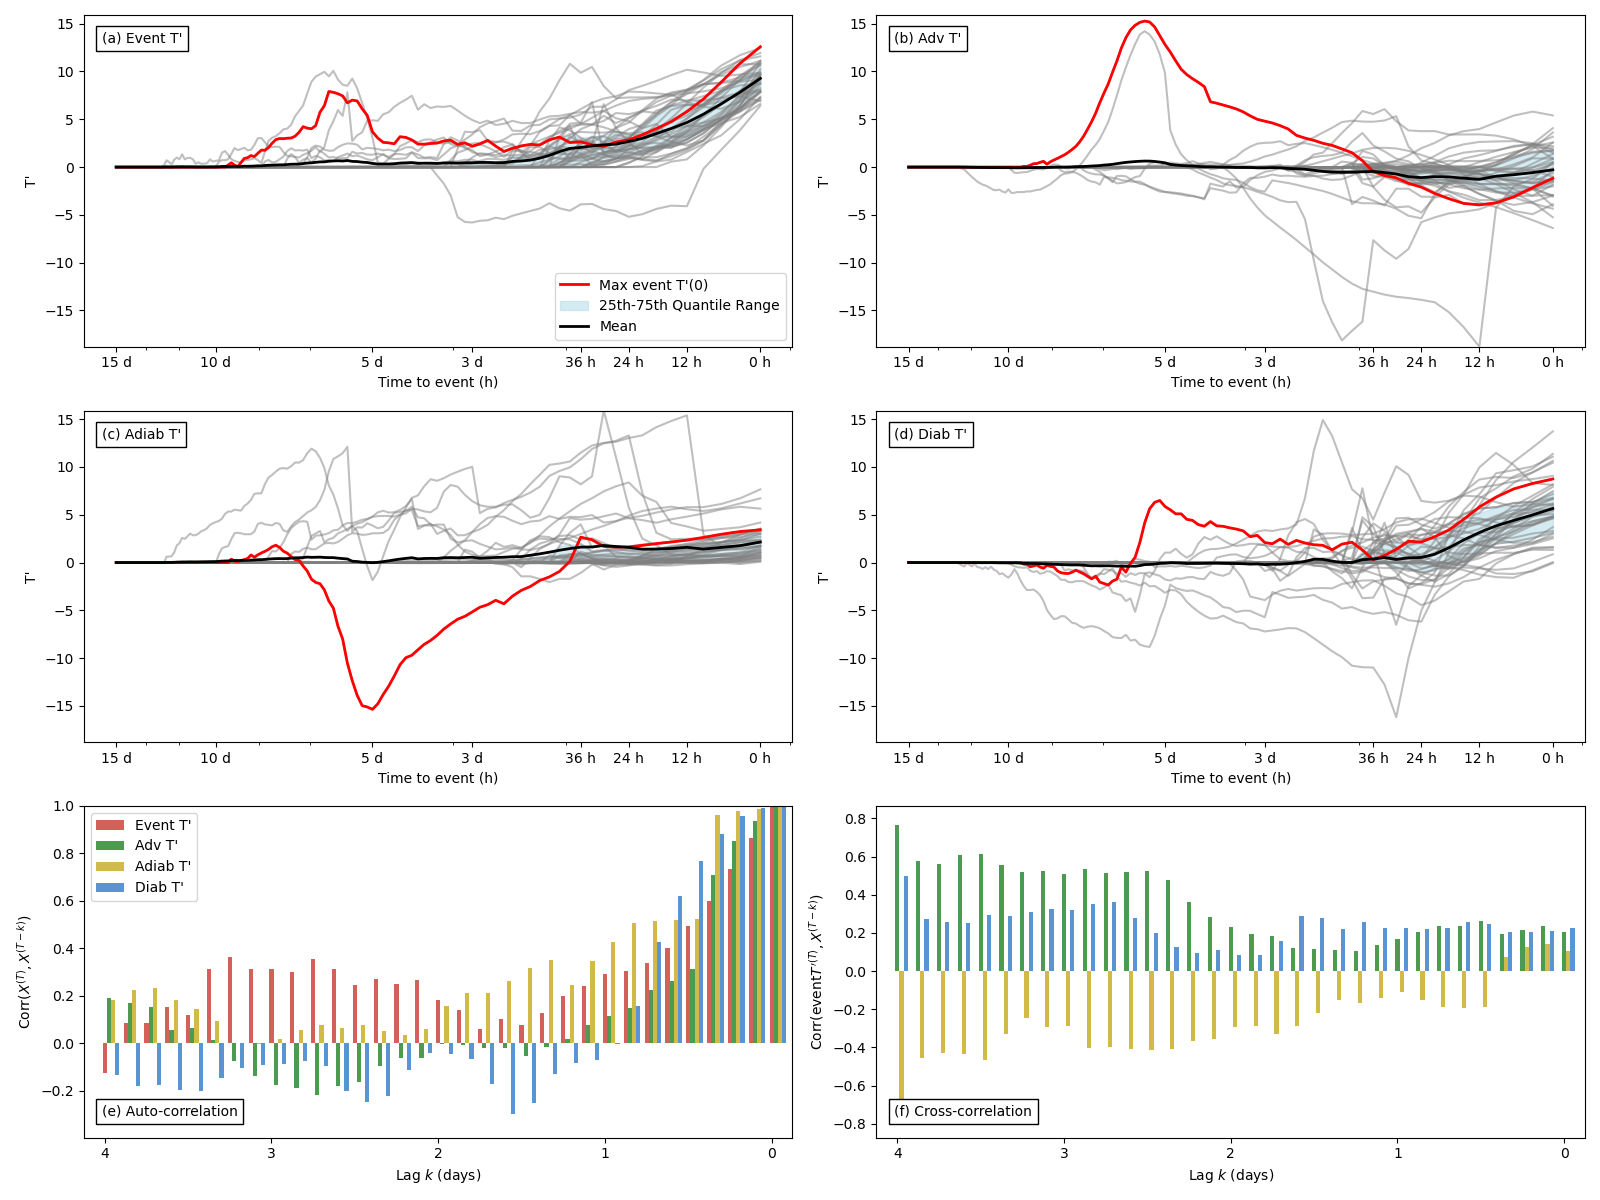
\includegraphics[width=0.9\textwidth]{images/sup3.png}
\end{figure}

\section{Differenced timeseries data}

%%% Local Variables: 
%%% mode: latex
%%% TeX-master: "MasterThesisSfS"
%%% End: 
